\chapter{Curve fitting of potential for MMO without photoemission}
\label{sec:second-app}
\newenvironment{longlisting}{\captionsetup{type=listing}}{}

From chapter \cref{sec:results} it became apparent from the plot of the potential of the MMO spacecraft over time in the cases where photoemission was not included that a convergence to a floating potential had not been achieved. In this appendix we present a Python script for curve fitting these timeseries plots of potential in order to estimate the floating potential that PINC would eventually converge to.


Three functions where optimized to fit against the absolute value of the potential:

\begin{subequations}
    \begin{align}
        \text{Hill function:} y(x) &= \frac{}{}\label{eq:Hill} \\
        \text{Exponential function:} y(x) &= a \exp{-b x} - c \label{eq:expFit} \\
        \text{Generalized logistic function} y(x) &=  A + \frac{K - A}{\left(C + Q e^{-B x}\right)^{\frac{1}{\nu}}}
    \end{align}
\end{subequations}


\begin{center}
\begin{figure}[H]
  \begin{subfigure}[b]{0.61\textwidth}
    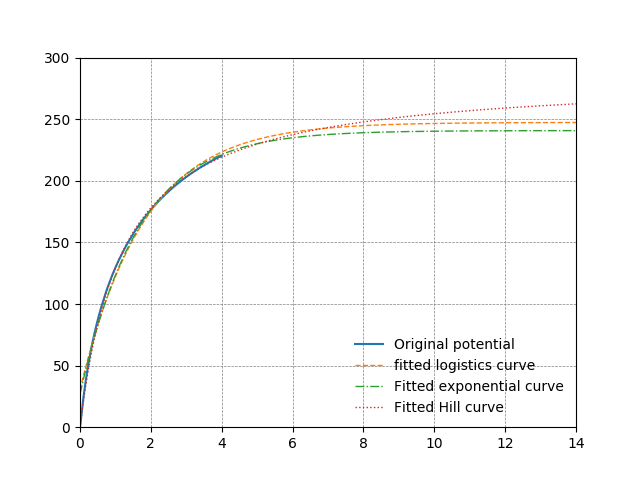
\includegraphics[width=\textwidth]{figures/Appendix/C_fit_NB.png}
    \caption{14,000 timesteps}
    \label{fig:C_fit_NB}
  \end{subfigure}
  \hfill
  \begin{subfigure}[b]{0.61\textwidth}
    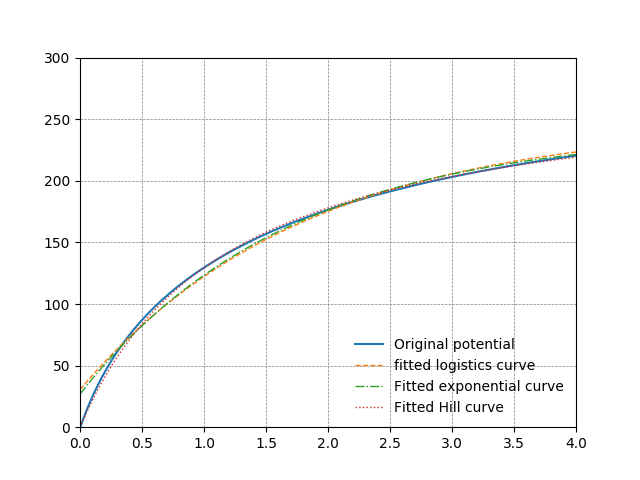
\includegraphics[width=\textwidth]{figures/Appendix/C_fit_NB_lim.png}
    \caption{4,000 timesteps}
    \label{fig:C_fit_NB_lim}
  \end{subfigure}
  \label{fig:Pot_noPH}
  \caption{Curve fitting using a generalized logistic function, Hall function, and exponential function of the potential of the MMO spacecraft without booms}
\end{figure}
\end{center}

\begin{center}
\begin{figure}[H]
  \begin{subfigure}[b]{0.61\textwidth}
    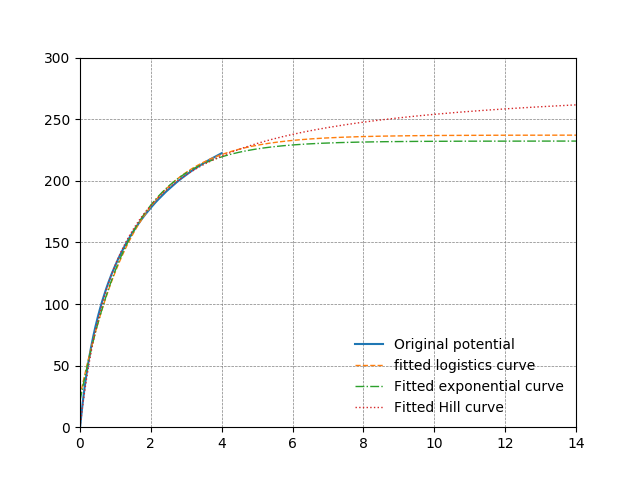
\includegraphics[width=\textwidth]{figures/Appendix/C_fit_WB.png}
    \caption{14,000 timesteps}
    \label{fig:C_fit_NB}
  \end{subfigure}
  \hfill
  \begin{subfigure}[b]{0.61\textwidth}
    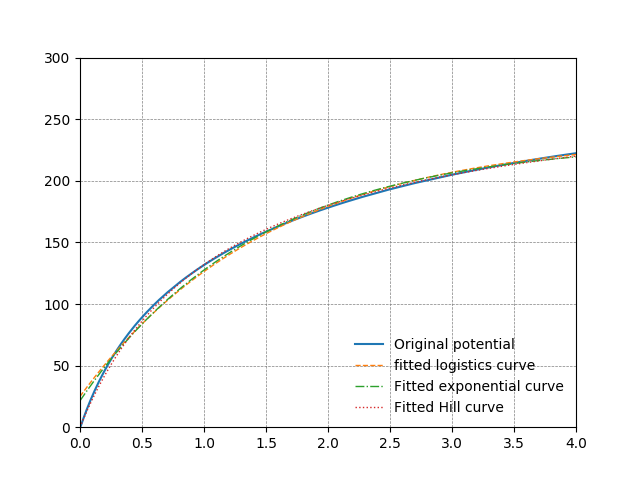
\includegraphics[width=\textwidth]{figures/Appendix/C_fit_WB_lim.png}
    \caption{4,000 timesteps}
    \label{fig:C_fit_NB_lim}
  \end{subfigure}
  \label{fig:Pot_noPH}
  \caption{Curve fitting using a generalized logistic function, Hall function, and exponential function of the potential of the MMO spacecraft with booms}
\end{figure}
\end{center}


\begin{longlisting}
\inputminted[
frame=lines,
framesep=2mm,
fontsize=\small
]{Python}{noPH_polyfit.py}
\caption{Dummy text}
\label{lst:polyfit}
\end{longlisting}